% !TEX root = ../main.tex



\section{Experiments}
\label{sec:experiments}

\subsection{Experimental Setup}
\label{sec:setup}

\noindent\textbf{Benchmarks.} We evaluate on three open-ended task streams (Table~\ref{tab:bench_stats}): \emph{PolyBench} for prediction markets~\cite{cheng2026polybench}, \emph{CTF-Dojo} for security challenges~\cite{zhuo2025training}, and \emph{FutureX} for event forecasting~\cite{zeng2025futurex}. All three enforce strict temporal order and covers the three dimensions of challenge. Details and non-stationarity diagnostics are in Appendix~\ref{app:benchmarks} and~\ref{app:nonstationarity}.

\begin{table}[!t]
\centering
\footnotesize
\setlength{\tabcolsep}{2pt}
\caption{Benchmark statistics for the three chronological task streams. Interval denotes the temporal ordering granularity used during evaluation.}
\label{tab:bench_stats}
\resizebox{\columnwidth}{!}{%
\begin{tabular}{@{}lrlll@{}}
\toprule
Bench. & Tasks & Span & Interval & Domain \\
\midrule
PolyBench & 5{,}075 & Feb 6--22, 2026 & Daily & Prediction markets \\
CTF-Dojo  & 261   & 2011--2024 & Year & Security \\
FutureX   & 503   & Jan--Apr 2026 & Weekly & Forecasting \\
\bottomrule
\end{tabular}
}
\end{table}

\noindent\textbf{Solver and evolver.} We use Claude Sonnet 4.6 as the solver for all experiments unless specified, and use Claude Opus 4.6 as the evolver, both at temperature 0 to attribute gains to the evolution algorithm rather than sampling noise; the no-evolution controls additionally report base-agent results for DeepSeek and Kimi. All algorithms share the same batch size (100/20/20 for PolyBench/CTF-Dojo/FutureX), batch loop, and temporal-reveal gate; only the evolution algorithm varies.

\noindent\textbf{Metrics.} Each benchmark reports metrics tailored to its deployment goal. PolyBench reports coverage, all-task accuracy, and total portfolio return. For CTF-Dojo and FutureX, we report the official pass rate (Pass@1) defined by the original benchmarks~\cite{zhuo2025training,zeng2025futurex}. Full definitions are in Appendix~\ref{app:benchmarks}.\zw{need to come back later}

\noindent\textbf{Baselines.} We compare against systems grouped as in Table~\ref{tab:rq1_main}. The no-evolution controls are base agents using \textbf{Sonnet}~\cite{}, \textbf{DeepSeek}~\cite{}, and \textbf{Kimi}~\cite{}. We compare with five auto-harness baselines: \textbf{A-Evolve}~\cite{aevolve}, \textbf{GEPA}~\cite{gepa2025}, \textbf{Meta-Harness}~\cite{metaharness2026} (archive-based proposer, $k{=}1$), \textbf{Continual Harness}, and \textbf{SkillOS}. We also compare with one human-designed system \textbf{OctoTools}~\cite{octotools2026}.

\noindent\textbf{Research questions.}
\textbf{RQ1} (\S\ref{sec:main-results}): How does Adaptive Auto-Harness compare against existing auto-harness systems on open-ended task streams?
\textbf{RQ2} (\S\ref{sec:barriers}): How does Adaptive Auto-Harness address benchmark-specific bottlenecks?
\textbf{RQ3} (\S\ref{sec:ablation}): Does stateful multi-agent evolution with evaluation feedback provide additional gains?
\textbf{RQ4} (\S\ref{sec:navloss}): Can solve-time routing effectively leverage specialized harness branches?
\textbf{RQ5} (\S\ref{sec:hitl}): Can human steering help when history provides insufficient signal?

\subsection{Comparison with Baselines}
\label{sec:main-results}

\begin{table*}[!t]
\centering
\caption{Main comparison across no-evolution agents, auto-harness baselines, a human-designed system, and our two variants. Bold marks the best result per metric and underline marks second best.}
\label{tab:rq1_main}
\begingroup
\small
\setlength{\tabcolsep}{3pt}
\def\arraystretch{1.12}
\resizebox{\textwidth}{!}{%
\begin{tabular}{@{}llcccccccccccc@{}}
\toprule
\multicolumn{2}{c}{} &
\multicolumn{3}{c}{\textbf{No evolution}} &
\multicolumn{5}{c}{\textbf{Auto-harness baselines}} &
\multicolumn{1}{c}{\textbf{Human}} &
\multicolumn{3}{c}{\textbf{Ours}} \\
\cmidrule(lr){3-5} \cmidrule(lr){6-10} \cmidrule(lr){11-11} \cmidrule(lr){12-14}
\textbf{Benchmark} & \textbf{Metric} &
\textbf{Sonnet} &
\textbf{DeepSeek} &
\textbf{Kimi} &
\textbf{A-Evolve} &
\textbf{GEPA} &
\makecell{\textbf{Meta}\\\textbf{Harness}} &
\makecell{\textbf{Cont.}\\\textbf{Harness}} &
\textbf{SkillOS} &
\textbf{OctoTools} &
\makecell{\textbf{Multi}\\\textbf{agent}} &
\textbf{Nav.} &
\makecell{\textbf{Full}\\\textbf{System}} \\
\midrule
\multirow{3}{*}{\textbf{PolyBench}}
& Coverage {\scriptsize$\uparrow$} & 31.7 & -- & -- & 21.1 & 32.6 & 55.3 & 10.4 & 24.1 & 54.4 & \underline{95.8} & 91.4 & \textbf{98.2} \\
& Accuracy {\scriptsize$\uparrow$} & 22.2 & -- & -- & 18.4 & 13.4 & 50.8 & 8.5 & 21.4 & 40.0 & \underline{79.8} & 77.4 & \textbf{80.9} \\
& Return {\scriptsize$\uparrow$} & $+$1.8 & -- & -- & $+$7.2 & $+$0.3 & $+$320 & $+$1.7 & $+$3.6 & $+$20.4 & \underline{$+$351} & \textbf{$+$352} & $+$331 \\
\midrule
\textbf{CTF-Dojo} & Pass {\scriptsize$\uparrow$} & 37.2 & -- & -- & 45.2 & 42.9 & 41.0 & 25.7 & 29.5 & 38.3 & \underline{47.9} & 46.0 & \textbf{50.2} \\
\midrule
\textbf{FutureX} & Pass {\scriptsize$\uparrow$} & 31.0 & -- & -- & \underline{47.5} & 28.2 & 29.4 & 31.8 & 29.8 & 25.6 & \textbf{49.5} & 44.1 & -- \\
\bottomrule
\end{tabular}
}
\endgroup
\vspace{-0.25em}
\end{table*}

\zw{revisit}
Table~\ref{tab:rq1_main} reports the main comparison. The central pattern is not that one baseline is weak, but that each baseline fails under a different deployment pressure. A-Evolve is competitive on the pass-rate benchmarks, reaching 45.2 on CTF-Dojo and 47.5 on FutureX, yet it covers only 21.1\% of PolyBench markets and therefore misses most trading opportunities. Meta-Harness is the strongest baseline on PolyBench return, but does not translate that advantage to CTF-Dojo or FutureX pass rates. OctoTools, the frozen human-designed system, is stable but lacks the stream-specific adaptation needed to lead any metric.

Our three variants cover complementary regimes. The Full System combines stateful multi-agent evolution with solve-time routing and is the strongest reliability-oriented configuration: it reaches 98.2\% PolyBench coverage with 80.9\% accuracy and leads CTF-Dojo at 50.2\%. The multi-agent evolver alone is the next-best system on PolyBench coverage/accuracy and leads FutureX at 49.5\%. Navigation alone is most valuable when payoff depends on selecting the right specialized branch: it achieves the highest PolyBench return while retaining high coverage and accuracy.

Reading the table by benchmark makes the deployment pressure sharper. On PolyBench, the Full System expands coverage to 98.2\%, far above the strongest non-ours coverage result (55.3\%), while navigation alone still slightly leads return because payoff depends on selecting the right specialized branch and confidence policy. On CTF-Dojo, the Full System clears the strongest baseline (A-Evolve at 45.2) by 5.0 points, with the multi-agent variant just behind at 47.9 and navigation alone at 46.0. On FutureX, the multi-agent system attains the highest pass rate at 49.5\%, two points above the strongest baseline.

\subsection{Benchmark Bottlenecks}
\label{sec:barriers}

\begin{figure}[!t]
\centering
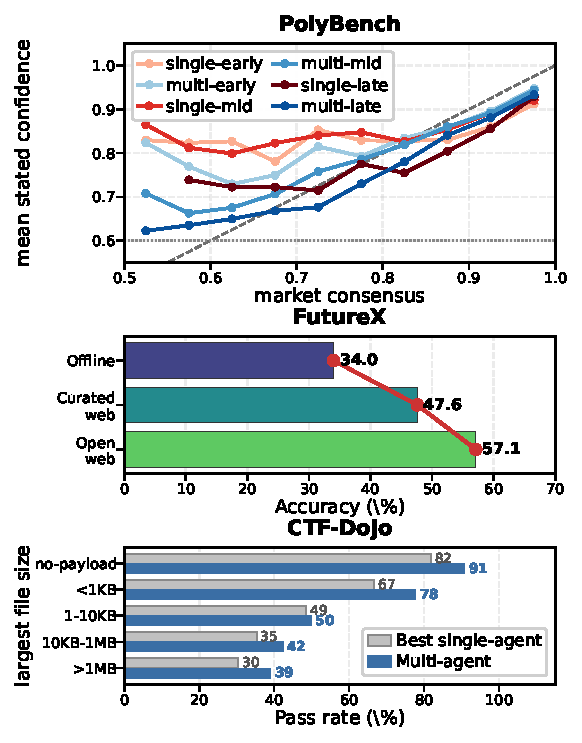
\includegraphics[width=\linewidth]{figures/l_evo_evidence.pdf}
\caption{$\Levo$ evidence across benchmark-specific bottlenecks. PolyBench stresses confidence calibration, FutureX stresses web-retrieval access, and CTF-Dojo stresses payload handling of different file sizes.}
\label{fig:l_evo_evidence}
\end{figure}

\begin{figure}[!t]
\centering
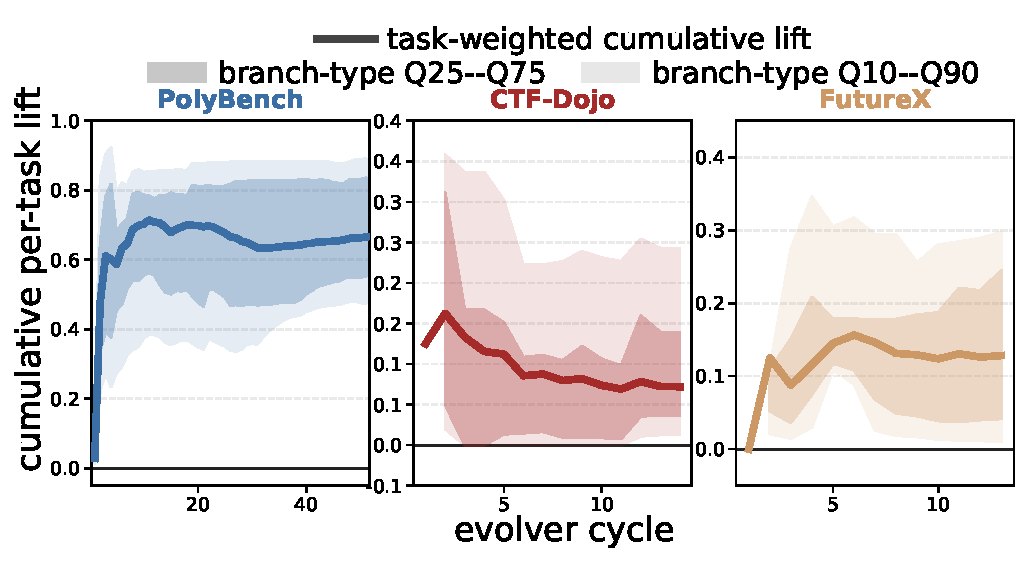
\includegraphics[width=\linewidth]{figures/l_adapt_evidence.pdf}
\caption{$\Ladapt$ evidence from branch specialization. Curves show cumulative routing lift over the baselines, while shaded bands show harness branch performance spread across cycles.}
\label{fig:l_adapt_evidence}
\end{figure}

RQ2 asks whether Adaptive Auto-Harness targets the bottlenecks that actually limit each benchmark. Figure~\ref{fig:l_evo_evidence} uses benchmark-specific stressors to expose the required constructed capabilities. On PolyBench, useful harnesses must calibrate confidence against market consensus: the multi-agent curves move upward with consensus, while weaker single-agent variants remain much flatter and under-use high-consensus opportunities. On FutureX, accuracy changes almost monotonically with retrieval access, showing that forecasting quality depends on source acquisition and web-search tooling rather than reasoning alone. On CTF-Dojo, payload size exposes a different bottleneck: multi-agent pass rate drops from $91\%$ on no-payload tasks to $39\%$ above 1MB, and the best single-agent line has the same downward shape. These panels show that the system must construct different capabilities for different benchmarks: confidence calibration for markets, search/source tools for forecasting, and payload-handling infrastructure for security tasks.

Figure~\ref{fig:l_adapt_evidence} shows the cumulative lift with adaptive-harness routing compared against the baselines and the quantile shows the performance across different branches. If a single committed harness were enough, routing lift over the median branch would collapse toward zero and branch-type quantiles would converge. Instead, lift remains positive across cycles, and the final-cycle branch-type IQRs stay wide: 28\% on PolyBench, 10\% on CTF-Dojo, and 20\% on FutureX. The adaptation bottleneck is especially clear on PolyBench, where category- and payoff-sensitive branches produce persistent lift, and on FutureX, where the positive lift coexists with the main-table Trend failure.

\subsection{Stateful Multi-Agent Evolution}
\label{sec:ablation}


\begin{figure}[!t]
\centering
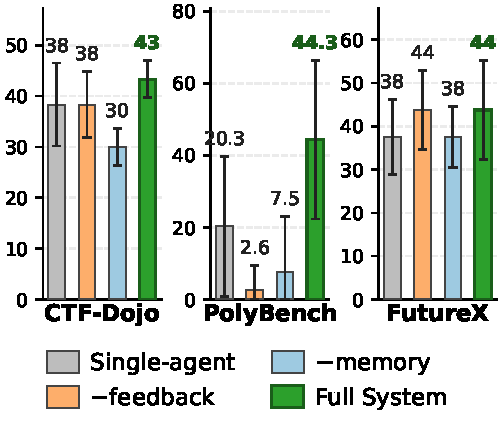
\includegraphics[width=\linewidth]{figures/figure_rq2.pdf}
\caption{Ablations for multi-agent evolution. Removing evaluation feedback or cross-cycle memory degrades end-of-stream performance relative to the full stateful system.}
\label{fig:rq2_stats}
\end{figure}

\begin{figure}[!t]
\centering
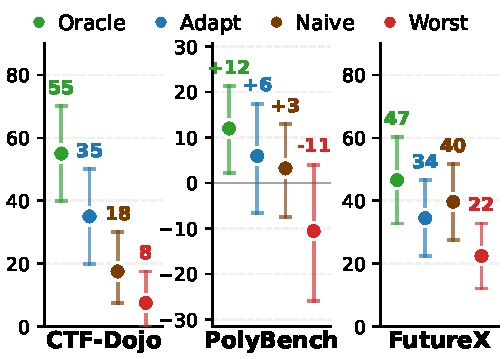
\includegraphics[width=\linewidth]{figures/figure_rq3.pdf}
\caption{Solve-time routing evaluation on a evolved harness tree. Oracle reports the best branch performance per task, Adapt uses our agentic router, Naive always uses \texttt{main} workspace, and Worst reports the worst branch performance per task.}
\label{fig:rq3_stats}
\end{figure}

\begin{figure*}[!t]
\centering
\begin{minipage}[t]{0.64\textwidth}
\centering
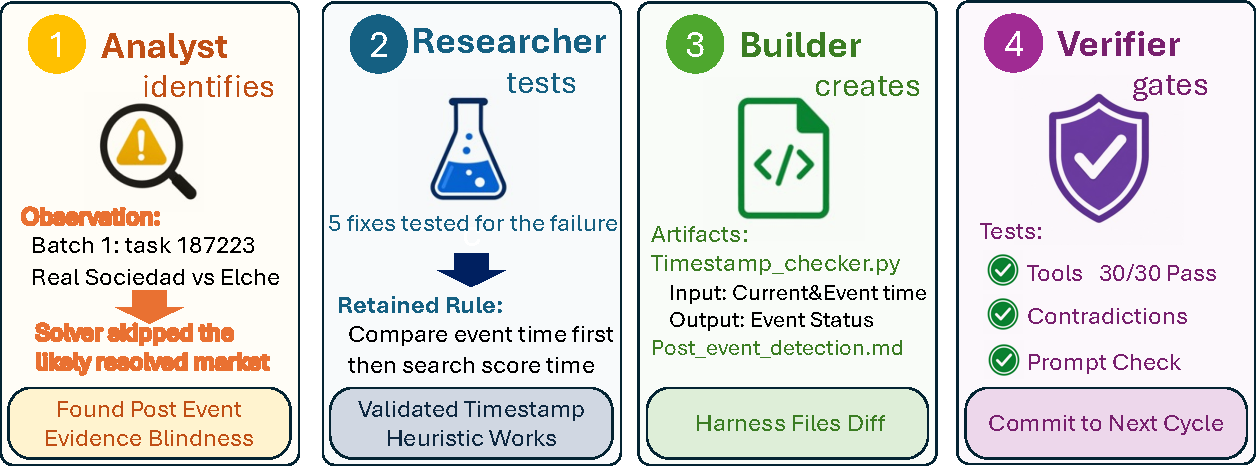
\includegraphics[width=\linewidth]{figures/rq2_demo_horizontal.pdf}\\[-0.2em]
{\scriptsize (a) Example of the four-phase evolution cycle. \zw{revisit}}
\end{minipage}\hfill
\begin{minipage}[t]{0.32\textwidth}
\centering
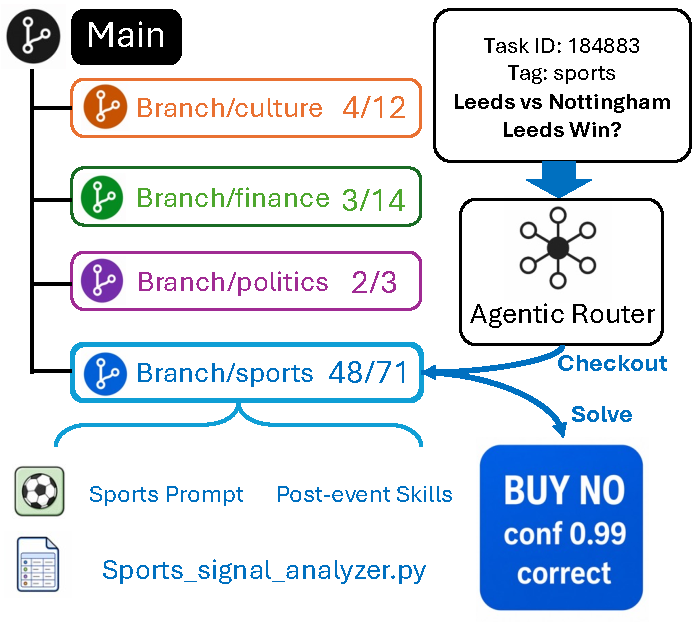
\includegraphics[width=\linewidth]{figures/rq3_demo.pdf}\\[-0.2em]
{\scriptsize (b) Example of the solve-time routing trace.}
\end{minipage}
\vspace{0.25em}

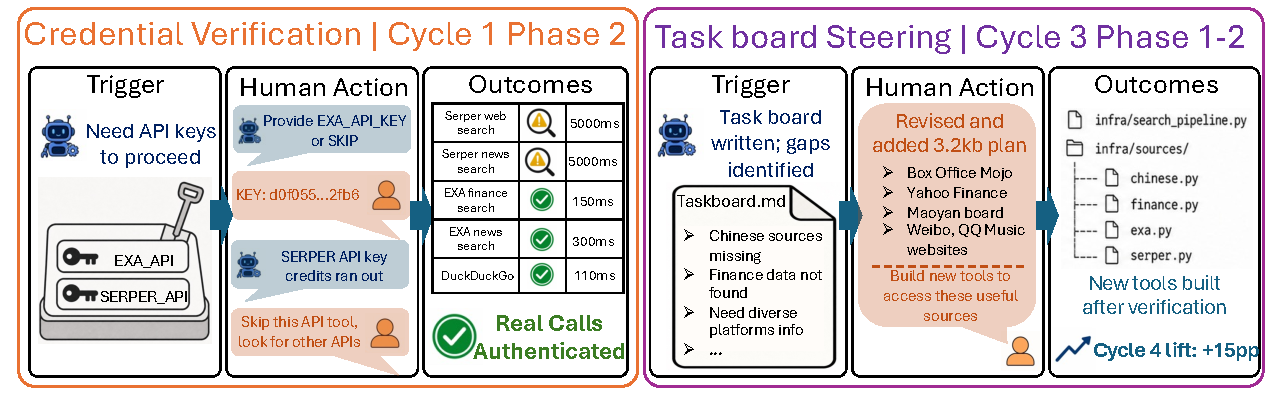
\includegraphics[width=\textwidth]{figures/rq4_demo_horizontal.pdf}\\[-0.2em]
{\scriptsize (c) Example of the Human-in-the-Loop workflow.}
\caption{Extracted trajectories of the designed multi-agent evolution, agentic routing, and Human-in-the-Loop.}
\label{fig:mechanism_traces}
\vspace{-0.4em}
\end{figure*}


RQ3 asks whether stateful multi-agent evolution with evaluation feedback provides additional gains. Figure~\ref{fig:rq2_stats} answers yes: compared with the full system, removing feedback collapses PolyBench CWR from $44.3$ to $2.6$, while removing memory lowers CTF-Dojo from $43\%$ to $30\%$ and FutureX from $44\%$ to $38\%$. These drops show that the gains come from the stateful interface to the stream: delayed outcomes must enter later evolution steps, and reusable exploit artifacts, parsing rules, and source heuristics must persist across cycles. Without these state channels, a multi-agent loop can still propose variants, but it cannot reliably turn stream evidence into stronger harnesses.



\subsection{Solve-Time Routing on the Harness Tree}
\label{sec:navloss}

RQ4 asks whether solve-time routing can leverage the specialized branches created by evolution. To isolate routing from construction, all strategies use the same evolved harness tree (Figure~\ref{fig:rq3_stats}; trace in Figure~\ref{fig:mechanism_traces}(b)): \emph{Oracle} chooses the per-task best branch, \emph{Adapt} uses our router, \emph{Naive} always uses \texttt{main}, and \emph{Worst} chooses the per-task worst branch. The answer is mostly yes: Oracle--Naive gaps show that branch specialization matters ($37\%$ on CTF-Dojo, $+9$ CWR on PolyBench, and $7\%$ on FutureX), and Adapt converts this specialization into gains on CTF-Dojo ($18\% \to 35\%$) and PolyBench ($+3 \to +6$ CWR). FutureX is the exception: Adapt trails Naive ($34\%$ vs.\ $40\%$) even though Oracle reaches $47\%$, showing that useful branches exist but the router does not identify them reliably under fast source shifts.

\subsection{Human Steering for Auto-Harnessing}
\label{sec:hitl}

\begin{figure}[!t]
\centering
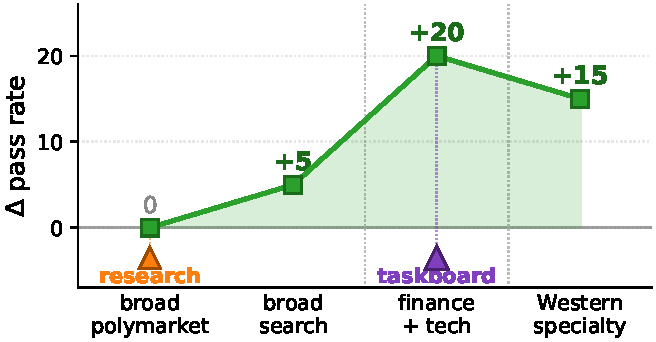
\includegraphics[width=0.95\linewidth]{figures/figure_rq4_timeline.pdf}
\caption{FutureX pass-rate lift with human steering. HITL is triggerd twice at different cycle phases (Research phase at cycle 1; Analyze phase at cycle 3). Cycle 1 starts with the zero lift and then improve on later cycles. The detailed trajectories is recorded in Figure~\ref{fig:mechanism_traces}.s}
\label{fig:rq4_hitl_passrate}
\end{figure}

RQ5 asks whether human steering helps when the stream history lacks the signal needed to build the next harness. We test this on FutureX because several failures come from missing search access or source-specific endpoint knowledge rather than from ordinary reasoning errors. Human input is therefore restricted to steering the auto-harness process: providing credentials when a research tool is blocked, or editing the task board with source directions that the evolver cannot infer from past trajectories. Figure~\ref{fig:mechanism_traces}(c) shows these two trigger types.

The answer is positive only when the steering targets the missing signal. In Figure~\ref{fig:rq4_hitl_passrate}, generic Polymarket transfer gives no lift, so the gains are not from adding arbitrary human advice. Broad search steering adds $+5\%$, while task-board steering adds $+20\%$ on finance/technology and $+15\%$ on Western-specialty slices. These gains are localized to the slices where the missing source access or source map matters. Thus, human steering is useful for auto-harnessing when it supplies external information absent from history; it is not a substitute for labeling tasks or manually choosing branches.
